
%%%%%%%%%%%%%%%%%%%%%%%%%%%%%%%%%%%%%%%%%%%%%%%%%%%%%%%%%%%%%%%%%%%%%%%
%%%%%%%%%%%%%%%%%%%%%%%%%%%%%%%%%%%%%%%%%%%%%%%%%%%%%%%%%%%%%%%%%%%%%%% 
%%%%%%%%%%%       								 Preamble				         	                                                        %%%%%%%%%% 
%%%%%%%%%%%%%%%%%%%%%%%%%%%%%%%%%%%%%%%%%%%%%%%%%%%%%%%%%%%%%%%%%%%%%%% 
%%%%%%%%%%%%%%%%%%%%%%%%%%%%%%%%%%%%%%%%%%%%%%%%%%%%%%%%%%%%%%%%%%%%%%% 
\documentclass[10pt]{beamer}
\usepackage{setspace}
\usepackage{color}
\usepackage{amsmath,lmodern}
\usepackage{hyperref}
\usepackage{graphicx}
\usepackage{multirow}
\usepackage{tikz}
\usetikzlibrary{fit,shapes.misc}
\usepackage{pdflscape}
\usepackage{amsmath}
\usepackage{lscape}
\usepackage{multirow}
\usepackage{enumerate}
\usepackage{epstopdf}
\usepackage{pdfpages}
\usepackage{appendixnumberbeamer}
\usepackage{color,soul}
\usepackage{grffile}
\usepackage{float}
\usepackage{relsize}
\usepackage{tcolorbox}
\newcounter{nodemarkers}
\usepackage{tikz}
\newcommand{\toplinesmall}{%
  \tikz[remember picture,overlay] {%
    \draw[blue,thick] ([yshift=-1cm, xshift=.9cm]current page.north west)
             -- ([yshift=-1cm,xshift=3.6cm]current page.north west);}}
             
\newcommand{\toplinemedium}{%
  \tikz[remember picture,overlay] {%
    \draw[blue,thick] ([yshift=-1cm, xshift=.9cm]current page.north west)
             -- ([yshift=-1cm,xshift=6.2cm]current page.north west);}}
 
 \newcommand{\toplinelarge}{%
  \tikz[remember picture,overlay] {%
    \draw[blue,thick] ([yshift=-1cm, xshift=.9cm]current page.north west)
             -- ([yshift=-1cm,xshift=8.9cm]current page.north west);}}           
             
 \newcommand{\toplinexlarge}{%
  \tikz[remember picture,overlay] {%
    \draw[blue,thick] ([yshift=-1cm, xshift=.9cm]current page.north west)
             -- ([yshift=-1cm,xshift=12cm]current page.north west);}}                       
             
\setbeamertemplate{footline}
{
  \leavevmode%
  \hbox{%
  \begin{beamercolorbox}[wd=.333333\paperwidth,ht=2.25ex,dp=1ex,center]{author in head/foot}%
    \usebeamerfont{author in head/foot}{\textcolor{blue}{ECON311}}
  \end{beamercolorbox}%
  \begin{beamercolorbox}[wd=.333333\paperwidth,ht=2.25ex,dp=1ex,center]{title in head/foot}%
    \usebeamerfont{title in head/foot}{\textcolor{blue}{Winter 2026}}
  \end{beamercolorbox}%
  \begin{beamercolorbox}[wd=.333333\paperwidth,ht=2.25ex,dp=1ex,right]{date in head/foot}%
    \usebeamerfont{date in head/foot}{\textcolor{blue}{Lecture 9 \: \: \: \: \: \: \: }
    \insertframenumber{} / \inserttotalframenumber\hspace*{2ex}} 
  \end{beamercolorbox}}%
  \vskip0pt%
}
\newtheorem{proposition}[theorem]{Proposition}

\newcommand\marktopleft[1]{%
    \tikz[overlay,remember picture] 
        \node (marker-#1-a) at (-0.2,1.2ex) {};%
}
\newcommand\markbottomright[1]{%
    \tikz[overlay,remember picture] 
        \node (marker-#1-b) at (0.16,-1ex) {};%
    \tikz[overlay,remember picture,thick,inner sep=4pt]
        \node[draw,rectangle,rounded corners, blue, fit=(marker-#1-a.center) (marker-#1-b.center)] {};%
}

\setbeamertemplate{caption}{\raggedright\insertcaption\par}
\setbeamertemplate{itemize items}[ball]
\setbeamertemplate{itemize subitem}[triangle]
\setbeamertemplate{itemize subsubitem}[triangle]
\tcbset{colframe=white,colback=white,nobeforeafter}
\beamertemplatenavigationsymbolsempty
\addtobeamertemplate{frametitle}{\vspace*{0.19cm}}{\vspace*{0cm}}


%%%%%%%%%%%%%%%%%%%%%%%%%%%%%%%%%%%%%%%%%%%%%%%%%%%%%%%%%%%%%%%%%%%%%%%
%%%%%%%%%%%%%%%%%%%%%%%%%%%%%%%%%%%%%%%%%%%%%%%%%%%%%%%%%%%%%%%%%%%%%%% 
%%%%%%%%%  									    Define Title									                                       %%%%%%%%%
%%%%%%%%%%%%%%%%%%%%%%%%%%%%%%%%%%%%%%%%%%%%%%%%%%%%%%%%%%%%%%%%%%%%%%%
%%%%%%%%%%%%%%%%%%%%%%%%%%%%%%%%%%%%%%%%%%%%%%%%%%%%%%%%%%%%%%%%%%%%%%% 
\title{ECON 311} 
\author{Lecture 9: Economics of Ideas}
\date{}
\AtBeginSection[]
{
 \begin{frame}<beamer>
 \tableofcontents[currentsection]
 \end{frame}
}
%%%%%%%%%%%%%%%%%%%%%%%%%%%%%%%%%%%%%%%%%%%%%%%%%%%%%%%%%%%%%%%%%%%%%%%
%%%%%%%%%%%%%%%%%%%%%%%%%%%%%%%%%%%%%%%%%%%%%%%%%%%%%%%%%%%%%%%%%%%%%%% 
%%%%%%%% 						     				Document								                                                %%%%%%%%
%%%%%%%%%%%%%%%%%%%%%%%%%%%%%%%%%%%%%%%%%%%%%%%%%%%%%%%%%%%%%%%%%%%%%%%
%%%%%%%%%%%%%%%%%%%%%%%%%%%%%%%%%%%%%%%%%%%%%%%%%%%%%%%%%%%%%%%%%%%%%%% 
\begin{document}
\setbeamercovered{transparent}

\begin{frame}
\maketitle
\end{frame}

%%%%%%%%%%%%%%%%%%%%%%%%%%%%%%%%%%%%%%%%%%%%%%%%%%%%%%%%%%%%%%%%%%%%%%%
%%%%%%%%%%%%%%%%%%%%%%%%%%%%%%%%%%%%%%%%%%%%%%%%%%%%%%%%%%%%%%%%%%%%%%% 
%%%%%%%% 						     				Introduction	             		                                		  %%%%%%%%
%%%%%%%%%%%%%%%%%%%%%%%%%%%%%%%%%%%%%%%%%%%%%%%%%%%%%%%%%%%%%%%%%%%%%%%
%%%%%%





\begin{frame}
\frametitle{\: \: \: Introduction }
\toplinemedium
\begin{itemize}
\item A large share of differences in $y$ across countries is due to differences in $\overline{A}$
\begin{itemize}
\vspace{.11in}
\item Differences in $\overline{A}$ are particularly important in understanding differences between rich and poor countries
\vspace{.11in}
\item Any policy aimed to reduce the gap between rich and poor countries needs to target the large differences in $\overline{A}$
\vspace{.11in}
\item To understand differences in $\overline{A}$, we need a model that does not treat TFP as an exogenous parameter 
\vspace{.11in}
\end{itemize}
\item The Romer Model incorporates differences in TFP by directly modeling the economics of ideas.
\begin{itemize}
\vspace{.11in}
\item Ideas are a different kind of input of production
\vspace{.11in}
\item The production of ideas is not free
\end{itemize}
\end{itemize}
\end{frame}

\begin{frame}
\frametitle{\: \: \: Ideas in the Production Function}
\toplinelarge
\begin{itemize}
\item Production of ideas result in changes in TFP:
\begin{eqnarray*} 
Y_t=F(K_t,L_t,A_t)=A_t \: K_t^{\frac{1}{3}} \: L_t^{\frac{2}{3}}
\end{eqnarray*}
\item There are constant returns to TFP
\begin{figure}
\centering
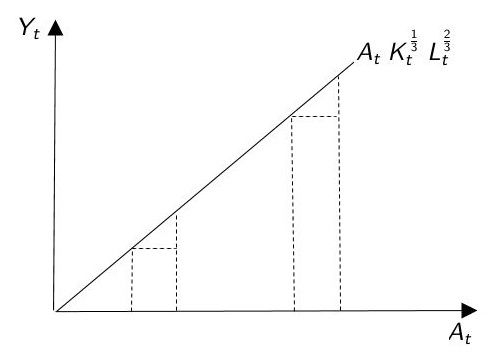
\includegraphics[scale=.55]{TFP_production_function}
\end{figure}
\end{itemize}
\end{frame}

\begin{frame}
\frametitle{\: \: \: Ideas in the Production Function}
\toplinelarge
\begin{itemize}
\item Production of ideas result in changes in TFP:
\begin{eqnarray*} 
Y_t=F(K_t,L_t,A_t)=A_t \: K_t^{\frac{1}{3}} \: L_t^{\frac{2}{3}}
\end{eqnarray*}
\item There are increasing returns to scale
\begin{itemize}
\vspace{.11in}
\item Multiply all inputs by a constant ($\gamma$):
\begin{eqnarray*} 
\begin{array}{l}
Y_t=F(\gamma \: K_t, \gamma \: L_t, \gamma \: A_t)=\gamma \: A_t \: \left(\gamma \:  K_t\right)^{\frac{1}{3}} \: \left(\gamma \: L_t\right)^{\frac{2}{3}} \\[3ex]
Y_t=\gamma ^2 \: F(K_t,L_t,A_t)
\end{array}
\end{eqnarray*}
\end{itemize}
\end{itemize}
\end{frame} 

\begin{frame}
\frametitle{\: \: \: The Production of Ideas}
\toplinelarge
\begin{itemize}
\item Producing ideas is not free:
\begin{itemize}
\vspace{.11in}
\item Innovators must invest ``labour'' to produce ideas:
\begin{eqnarray*}
\begin{array}{l}
L_{A_t}=\overline{l} \: \overline{L} \\[3ex]
L_{Y_t}=(1-\overline{l}) \: \overline{L} \\[3ex] 
L_{A_t}+L_{Y_t}=\overline{L}
\end{array}
\end{eqnarray*}
\item Trade-off between producing consumption goods and ideas:
\begin{eqnarray*}
\begin{array}{l}
Y_t=A_t \:  L_{Y_t}  \\[3ex]
A_{t+1}=A_{t}+\underbrace{\overline{z} \: A_t \: L_{A_t}}_{\text{Idea}}
\end{array}
\end{eqnarray*}
\end{itemize}
\end{itemize}
\end{frame}

\begin{frame}
\frametitle{\: \: \: TFP Growth}
\toplinemedium
\begin{itemize}
\item Accumulation of ideas result in TFP growth over the long-run:
\begin{eqnarray*}
\underbrace{\frac{A_{t+1}-A_t}{A_t}}_{\overline{g}}=\overline{z} \: \overline{l} \: \: \overline{L}
\end{eqnarray*}
\item \textcolor{red}{(Trade-off)} An increase in $\overline{l}$ increases $A_{t+1}$, but decreases $Y_t$ 
\begin{itemize}
\vspace{.11in}
\item An increase in $\overline{l}$ has the potential to increase output in the long-run
\vspace{.11in}
\item Furthermore, an increase in $\overline{l}$ increases the long-run growth rate of output 
\end{itemize}
\end{itemize}
\end{frame}

\begin{frame}
\frametitle{\: \: \: Output Growth in the Long-Run}
\toplinelarge
\begin{itemize}
\item Output per capite at time $t$ is:
\begin{eqnarray*}
y_t=A_0 \: (1-\overline{l}) \: (1+\overline{g})^t
\end{eqnarray*}
\item Using the growth rate of TFP, we can solve for the long-run growth of $y_t$ (BGP):
\begin{eqnarray*}
\begin{array}{c}
g_y=\overline{z} \: \overline{I} \: \overline{L} (1-\overline{I}) 
\end{array}
\end{eqnarray*}
\end{itemize}
\end{frame}

\begin{frame}
\frametitle{\: \: \: Trade-Off}
\toplinelarge
\begin{figure}
\centering
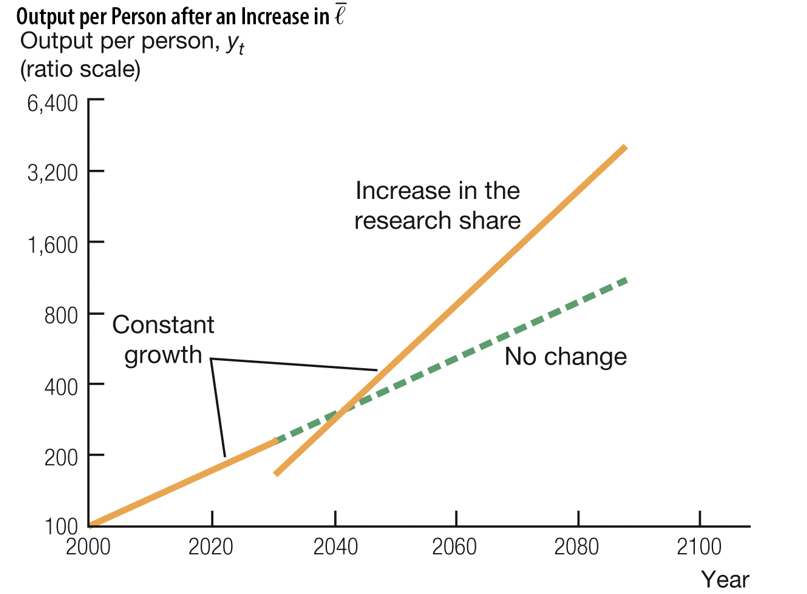
\includegraphics[scale=.35]{romer_trade}
\end{figure}
\end{frame}

\begin{frame}
\frametitle{\: \: \: Conclusion}
\toplinemedium
\begin{itemize}
\item Introducing the production of ideas ...
\begin{itemize}
\vspace{.11in}
\item provides a theory as to why, in the long-run, some countries are able to grow at a faster rate than others 
\vspace{.11in}
\begin{enumerate}
\item More labour allocated to the ideas producing sector
\vspace{.11in}
\item Countries have different ideas generating processes
\vspace{.11in}
\end{enumerate}
\item is consistent with the data because it models long-run growth in GDP per capita as the result of TFP growth  
\end{itemize}   
\end{itemize}
\end{frame}





\end{document}



